\begin{figure*}[t]
\centering
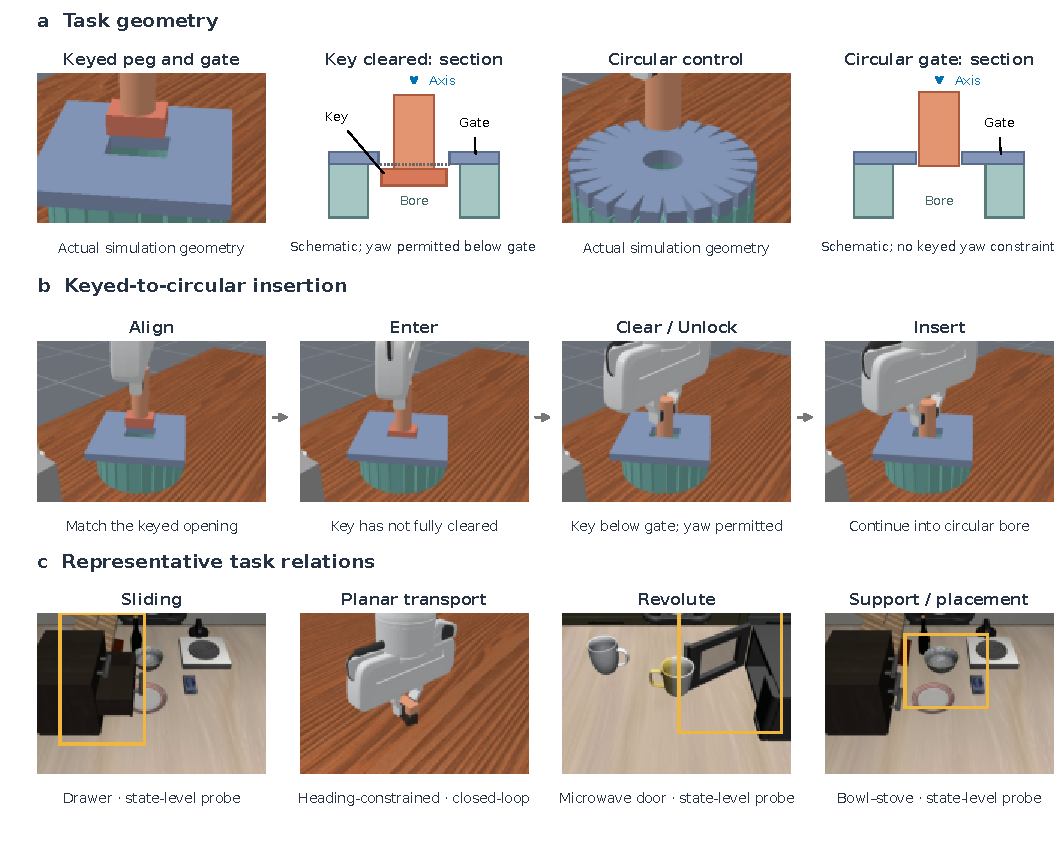
\includegraphics[width=\textwidth]{task_scene_overview.pdf}
\caption{Simulation geometry, insertion stages, and representative task relations. (a) Closeups replayed in the keyed and circular environments, paired with explicitly schematic sections of the gate and bore. The keyed section depicts the key after clearance; it is not a section of the adjacent alignment frame. Axial rotation becomes admissible below the keyed gate, whereas the circular control has no keyed yaw constraint. These geometric permissions do not prescribe a zero yaw-response coefficient. (b) Four states from one successful keyed rollout rendered with the same camera and crop. Key clearance is checked from the recorded pose and key geometry; Unlock denotes the controller phase following clearance. (c) Representative task relations. Planar transport replays the heading-constrained PlanarPush-v1 closed-loop benchmark, whose collector uses a guided grasp-and-slide procedure. Drawer, microwave and bowl scenes are controlled state-level probes; their visible robots are scene context rather than evidence of execution. Outlines locate objects in the state-level scenes. Panels are illustrative states, not quantitative success comparisons.}
\label{fig:task_scene_overview}
\end{figure*}
